\documentclass{beamer}

\usepackage{graphicx}

\newcommand {\framedgraphic}[2] {
    \begin{frame}{#1}
        \begin{center}
            \includegraphics[width=\textwidth,height=0.8\textheight,keepaspectratio]{#2}
        \end{center}
    \end{frame}
}

\title{Block Ciphers}
\begin{document}

\begin{frame}
	\titlepage
\end{frame}

\begin{frame}{Block Ciphers}
	\begin{block}{Definition}
		A block cipher is a deterministic algorithm operating on fixed-length
		groups of bits, called \textit{blocks}, with an unvarying transformation
		that is specified by a symmetric key.
	\end{block}
\end{frame}

\begin{frame}{Block Ciphers}
	\begin{block}{Definition}
		A block cipher is a \textbf{deterministic algorithm} operating on fixed-length
		groups of bits, called \textit{blocks}, with an unvarying transformation
		that is specified by a symmetric key.
	\end{block}

	\begin{block}
		Given the same input, a block cipher will always produce the same
		output.
	\end{block}
\end{frame}

\begin{frame}{Block Ciphers}
	\begin{block}{Definition}
		A block cipher is a deterministic algorithm operating on \textbf{fixed-length
		groups} of bits, called \textit{blocks}, with an unvarying transformation
		that is specified by a symmetric key.
	\end{block}

	\begin{block}{}
		A block cipher does not operate on arbitrarily-long data.
	\end{block}
\end{frame}

\begin{frame}{Block Ciphers}
	\begin{block}{Definition}
		A block cipher is a deterministic algorithm operating on fixed-length
		groups of \textbf{bits}, called \textit{blocks}, with an unvarying transformation
		that is specified by a symmetric key.
	\end{block}

	\begin{block}{}
		A block cipher does not operate on characters, but strings of bits.
	\end{block}
\end{frame}

\begin{frame}{Block Ciphers}
	\begin{block}{Definition}
		A block cipher is a deterministic algorithm operating on fixed-length
		groups of bits, called \textit{blocks}, with an unvarying transformation
		that is \textbf{specified by a symmetric key}.
	\end{block}

	\begin{block}{}
		A block cipher is a \textit{collection} of transformations, indexed by a
		key.
	\end{block}
\end{frame}

\begin{frame}{Block Ciphers}{A Functional Description}
	\begin{figure}
		\centering
		Block cipher:
		\[ E: \{0,1\}^k \times \{0,1\}^n \rightarrow \{0,1\}^n \]
		\[ D: \{0,1\}^k \times \{0,1\}^n \rightarrow \{0,1\}^n \]
		\visible<2->{
			\[ \forall K \in \{0,1\}^k: E_K = D_K^{-1} \]
		}
		%\[ E_K: \{0,1\}^n \rightarrow \{0,1\}^n \]
	\end{figure}

	\begin{block}{}
		\begin{itemize}
			\item A block cipher consists of two algorithms: one for encryption,
				$E$, and the other for decryption, $D$. Each take a key and a
				block, and produce a block of the same size.
			\visible<2->{
				\item For a given key, decryption must be the inverse of encryption.
			}
		\end{itemize}
	\end{block}

	%Question: For one-byte block, why is XOR cipher (OTP) not an option?
	% Answers: Because it's terrible
	%          Because you can't reuse key
	%          Because it doesn't stand up to anything stronger than COA
\end{frame}

\begin{frame}{Modes}
	In order to apply a block cipher to a string of data longer than its block
	size, we use a \textit{mode of operation}. We will get to those later.
\end{frame}

\begin{frame}{Security Assumptions}
	While previously we dealt with ciphertext-only attacks, there are many other
	attack prototypes that block ciphers (and mode) must defend against:

	\begin{itemize}
		\item Ciphertext-only distinguisher
		\item Ciphertext-only attack
		\item Known-plaintext attack
		\item Chosen-plaintext attack
		\item Chosen-ciphertext attack
	\end{itemize}

	They each have nuances and sub-types, but those four are the archetypical
	attack scenarios.

	\begin{block}{}
		There should be no apparent correlation between the plaintext and the
		ciphertext in the absence of the key, and yet it should be easy to
		invert, given the key.
	\end{block}
\end{frame}

\begin{frame}{Block Cipher Design}
	\begin{block}{}
		Most block ciphers are \textit{iterated}, alternating confusion and
		diffusion.

		We convert the given key into a sequence of \textit{round keys}, one
		$K_i$ for each round.

		\[ M_i = R_{K_i}(M_{i-1}) \]

		Usually there is some ramp-up transformation on either end, but that is
		not necessary.
	\end{block}

	Each round contains elements of \textit{confusion} (e.g. substitution
	cipher) and \textit{diffusion} (e.g. transposition cipher).

	Additionally, each round generally mixes the key into the data via some
	invertible operation, primarily XOR.

	Some ciphers use ADD/MINUS instead... why could this be a disadvantage?

	% Answer I'm looking for: timing issues wrt digital logic. But there are
	% many other problems here, too.

\end{frame}

\begin{frame}{Substitution-Permutation Network}
	\begin{minipage}{0.4\textwidth}
		\begin{figure}[h!]
			\centering
			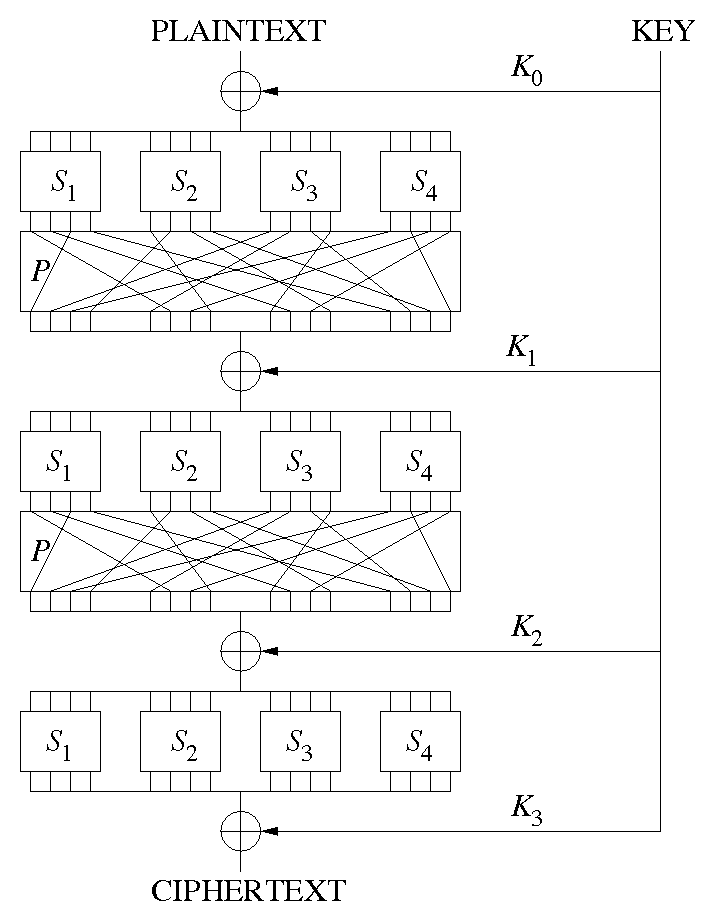
\includegraphics[width=\textwidth,height=0.8\textheight,keepaspectratio]{spn}
		\end{figure}
	\end{minipage}
	\begin{minipage}{0.4\textwidth}
		\begin{itemize}
			\item AES (Rijndael)
			\item 3-Way
			\item SAFER
			\item SHARK
			\item Square
		\end{itemize}
	\end{minipage}
\end{frame}

\begin{frame}{Feistel Network}
	\begin{minipage}{0.5\textwidth}
		\begin{figure}[h!]
			\centering
			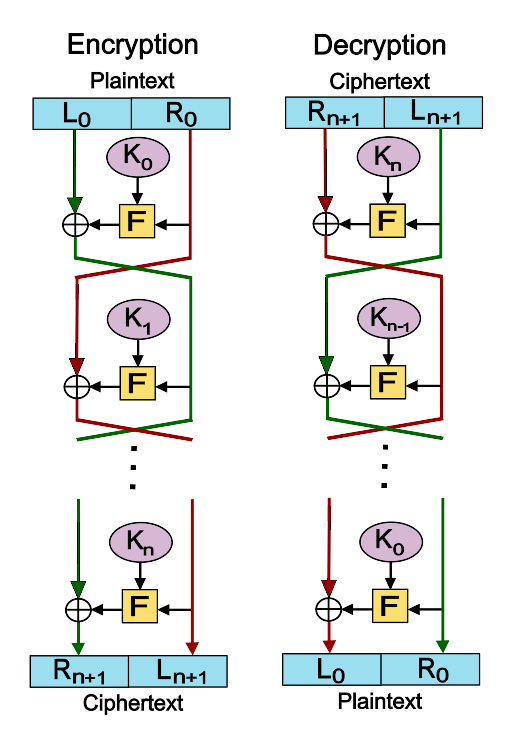
\includegraphics[width=\textwidth,height=0.8\textheight,keepaspectratio]{feistel-structure}
		\end{figure}
	\end{minipage}
	\begin{minipage}{0.4\textwidth}
		\begin{align*}
			L_i &= R_{i-1} \\
			R_i &= L_{i-1} \oplus F_{K_i}(R_{i-1})
		\end{align*}
		%Turns out, making nontrivial invertible functions is difficult.

		Advantage: encryption and decryption are very similar,
		usually only requiring a reversal of the key schedule.
	\end{minipage}

\end{frame}

\begin{frame}{Lai-Massey}
	\begin{figure}[h!]
		\centering
		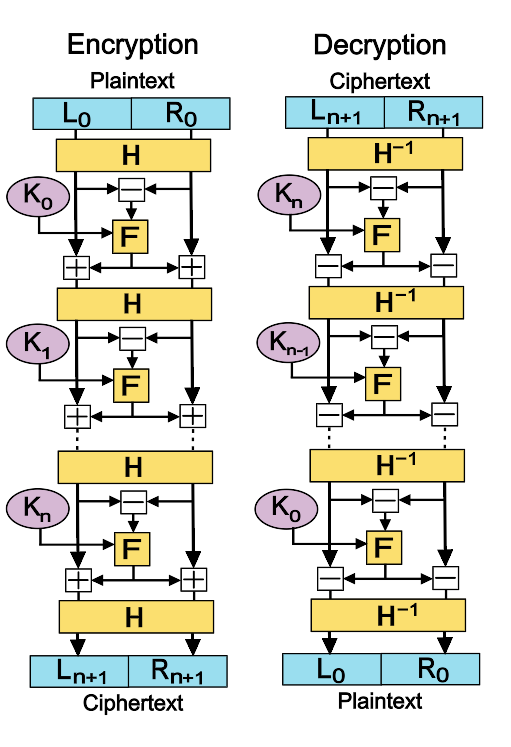
\includegraphics[width=\textwidth,height=0.8\textheight,keepaspectratio]{lai-massey}
	\end{figure}
\end{frame}

\begin{frame}
\end{frame}
\end{document}
